\section{Theorie}
\label{sec:Theorie}

Ziel dieses Versuches ist es, sich mit dem HeNe-Laser vertraut zu machen. Dafür werden zwei TEM-Moden des Lasers und die
Stabilitätsbedingung des Resonators untersucht. Desweiteren werden die Polarisation und die Wellenlänge des Lasers bestimmt. 

Das Wort \textit{Laser} ist eine Abkürzung für den englischen Begriff \textit{"Light Amplification by Stimulated Emission
of Radiation"}. Ein Laser besteht im Wesentlichen aus drei Komponenten, mit denen es möglich ist, den charakteristischen Laserstrahl zu
erzeugen. Diese Komponenten sind das aktive Lasermedium, die Pumpquelle und der Resonator, auf die im Folgenden näher 
eingegangen werden soll. 

\subsection{Aktives Lasermedium}

Im aktivem Lasermedium finden die optischen Übergänge statt, weswegen dieses das Strahlungsspektrum des Lasers bestimmt. Im Fall des
HeNe-Lasers fungiert das Neon als aktives Lasermedium. Zunächst wird die Wechselwirkung zwischen Stahlungsfeld und Lasermedium als 
Zweizustandsystem betrachtet. Es gibt demnach einen Grundzustand mit Besetzungszahl $n_1$ und einen angeregten Zustand mit Besetzungszahl
$n_2$. Die Wechselwirkung kann im Wesentlichen mit drei Prozessen beschrieben werden.

Die Absorption, bei der ein Photon ein Atom aus dem Grundzustand in den ersten angeregten Zustand hebt. \\
Die spontane Emission, bei der das Atom spontan aus dem angeregten Zustand zurück in den Grundzustand fällt, wobei ein Photon in 
beliebiger Richtung abgestrahlt wird. \\
Und die stimulierte Emission, bei der ein Atom im angeregten Zustand durch ein eingestrahltes Photon, zurück in den Grundzustand 
fallen kann. Hier hat das stimulierte Photon dann genau die Gleiche Richtung, Energie, Phasenlänge und Polarisation wie das 
eingestrahlte Photon. Das ist der relevante Prozess für einen Laser. \\
Diese Prozesse sind in Abbildung \ref{fig:prozesse} schematisch dargestellt. 

\begin{figure}[H]
    \centering
    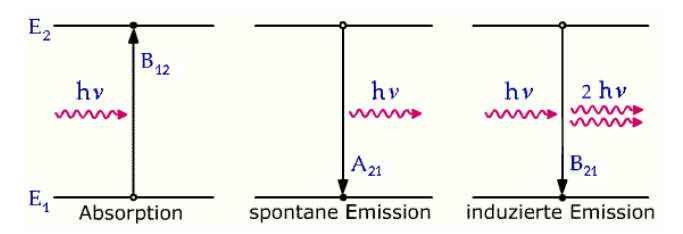
\includegraphics[scale=0.5]{content/prozesse.png}
    \caption{Schematische Darstelleung der relevanten Prozesse in einem Zweizustandsystem. \cite{prozess}}
    \label{fig:prozesse}
\end{figure}

Die Einsteinkoeffizienten $A_{21}$, $B_{21}$ und $B_{12}$ geben dabei ein Maß für die Übergangswahrscheinlichkeiten
an. 
Ein Laser lässt sich allerdings nicht komplett durch ein Zweizustandsystem beschreiben. Dies liegt daran, dass die Zustände
im thermischen Gleichgewicht der Maxwell-Boltzmann Verteilung folgen. Das führt dazu, dass maximal eine Gleichbesetzung der 
Zustände erreicht werden kann. Demnach wäre eine Besetzungsinversion nicht möglich, was aber das notwendige Kriterium für einen
Laser ist. 

\subsection{Die Pumpquelle}

Die Pumpquelle fügt dem System Energie hinzu und erzeugt damit die notwendige Besetzungsinversion. Dies funktioniert mit dem 
Prinzip des Optischen Pumpens. Im Fall des HeNe-Lasers ist das Pumpgas Helium, weswegen kein Zweizustandsystem mehr vorliegt. 
Dabei wird die Besetzungsinversion durch elektrische Entladung im Laserrohr erzeugt. Folgend geben die so angeregten Helium Atome 
ihre Anregungsenergie an die Neon Atome durch Stöße ab. Dies kann durch ein Niveauschema dargestellt werden, welches in 
Abbildung \ref{fig:pump} zu sehen ist. 

\begin{figure}[H]
    \centering
    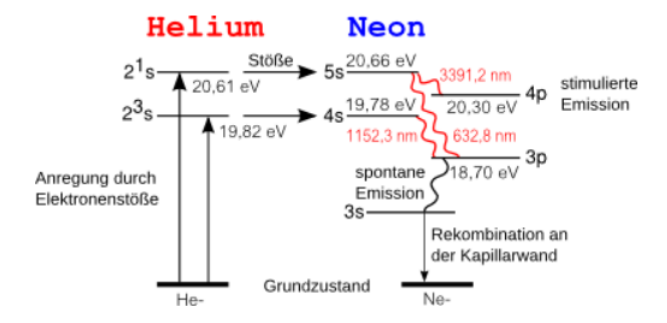
\includegraphics[scale=0.5]{content/pump.png}
    \caption{Niveauschema eines HeNe-Lasers. \cite{Zeugs}}
    \label{fig:pump}
\end{figure}

Es ist zu erkennen, dass die Laserlinie bei $\lambda = \SI{632.8}{\nano\metre}$ beim Übergang von 3s zu 2p am intensivsten ist. 

\subsection{Der Resonator}

Die Verstäkung des Lasers nimmt mit der Länge des Laufweges zu, weswegen ein Resonator diesen Laufweg verlängert. Der Resonator
besteht aus zwei Spiegeln, welche sich gegenüber stehen. Dabei ist einer totalreflektierend, während der andere eine geringe
Transmission zulässt, um die Auskopplung des Lasers zu ermöglichen. Dieses Prinzip ist in Abbildung \ref{fig:resonator} schmeatisch dargestellt.

\begin{figure}[H]
    \centering
    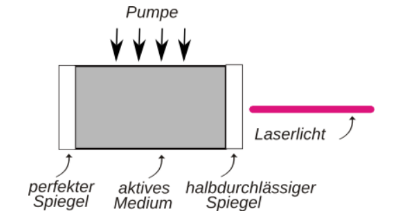
\includegraphics[scale=0.5]{content/Resonator.png}
    \caption{Schematische Darstellung eines Resonators. \cite{Zeugs}}
    \label{fig:resonator}
  \end{figure}

Die Unterscheidung zwischen Resonatoren erfolgt durch die verwendeten Spiegel. Häufig werden sphärische, planparallele oder eine 
Kombination dieser Spiegelarten eingesetzt. Ein Resonator wird dann als stabil bezeichnet, wenn die Verluste geringer als die 
Verstärkung durch stimulierte Emission sind. Die Stabilitätsbedingung ist dann 

\begin{equation}
    0 \leq g_1 g_2 \leq 1
    \label{eqn:Stabi}
\end{equation}

mit Parametern

\begin{equation*}
    g_i = 1 - \frac{\text{Resonatorlänge } L}{\text{Krümmungsradien Spiegel } r_i}.
\end{equation*}

In einem Resonator bilden sich stehende Wellen aus, die als Moden $TEM_{lqp}$ bezeichnet werden, wobei $q$ die longitudinale Mode 
und $l, p$ die transversalen Moden bezeichnen. Demnach wäre $TEM_{00}$ die Grundmode. Für diese hat die Intensität die Form 
einer Gaußkurve gemäß

\begin{equation*}
    I(r) = I_0 \exp{\left(\frac{-2r^2}{\omega ^2}\right)}.
\end{equation*}

Moden höherer Ordnung, wie $TEM_{00}$, werden allgemein als Multimoden bezeichnet. Diese machen sich durch unregelmäßige
Lichtintesität im Strahlprofil bemerkbar und stehen somit für eine schlechtere Stahlqualität. 

